\documentclass{IEEEtran}
\usepackage{amsmath}
\usepackage{hyperref}
\usepackage{graphicx}
\usepackage{listings}

\title{Building a Resilient Control Scheme over Unreliable Wireless Networks}
\author{Chandler Swift \\ ~ \\
  Spring--Fall 2019 \\
  Advisor: Dr. Peter A. H. Peterson \\
  Computer Science Department \\
  University of Minnesota Duluth
}

\begin{document}

\maketitle

\section{Introduction}
% TODO: don't announce the topic here.
The purpose of this study is to develop a method of network communication and
control of a remotely drivable research robot to enable effective network
control. This can be thought of as a specific example of the general problem
of establishing reliable communication over an unreliable network, such a
last-mile internet connection over failing cable or a satellite internet
connection, and will build off other efforts to minimize the effects of
latency such as those applied in game development\cite{reducinglag} and in other
cases such as Voice over IP calling\cite{briscoe2014reducing}.

Specifically, in our use case, we have difficulty reliably traversing campus
with the robot, as it must transition between access points. This task can take
potentally ten to fifteen seconds, in which time control and communication to
the robot are lost. The way the robot's control system was designed at the time
of the beginning of this research meant that the robot would continue to drive
even after connection was lost, potentially running into obstacles or
otherwise causing itself damage.

With the end goal of navigating across campus with resilience to changing
wireless access points, we will attempt to both minimize the time and the
effect of the transition between those access points by changing the
hardware and software networking configuration of the Raspberry Pi acting
as a network server for the robot.

\section{Methods}
Of the seven layers in the OSI networking model, there are several which we
can attempt to improve. We can refine the physical layer by providing additional or
more powerful wireless hardware, which should increase the duration we will
remain successfully connected to one access point, and minimize the frequency
and duration of such transitions. Secondly, because we have written our own
control protocol on top of the WebSocket protocol\cite{protocol}, we also 
explored modifications which can be made at the
protocol layer to minimize the disruptive effects of access point handovers.

We obtained three adapters for the hardware portion of this test. First, we
use the Canakit-branded wireless adapter that came bundled with a purchased
Raspberry Pi\cite{canakit}, which is built around a MediaTek RT5370 chipset,
and supported natively by the Linux kernel. Initially this adapter had been
directly connected to the Raspberry Pi inside the frame. However, given the
detrimental effect which the metal frame is likely to have on wireless 
performance from inside, the adapter was moved to use a USB extension and to
sit outside of the robot. Tests were run with this adapter both inside and
outside of the robot. Secondly, we purchased a BrosTrend high-gain dual-band
wireless adapter as a higher-end model to test\cite{brostrend} (built around
the Realtek 8812au chipset, which is supported natively by the Linux kernel
as of v4.19). To gain additional diversity in selection, we
purchased a third adapter: a TP-Link Archer T2UHP \cite{archer}. However,
we were unable to get this adapter to work with the Raspberry Pi, nor with
any other computer we tried, and so this was not used in any of the following
experiment.

With each adapter configuration (Canakit adapter inside the frame; Canakit
adapter mounted on the top of the robot; BrosTrend adapter mounted on top
of the robot), we proceeded to make runs down the length of the third
floor of Heller Hall. Runs were conducted during weekends, where there were
fewer people present to create additional traffic to potentially disturb
results. At a consistent speed of approximately one mile per hour (so chosen
due to this being approximately the top speed of the robot), the robot was
pushed down the hall while sending ICMP \texttt{echo} packets to a computer
on the building's wired network. From this, the response time, wall clock
time, and currently connected access point were measured, 5 times per second,
until the end of the hallway was reached. Each adapter was tested over the
course of four runs using a custom-written script\cite{hallway-script}.

We also tested protocol-layer improvements. This was done by adding a
watchdog timer function\cite{watchdog} into the Raspberry Pi's web server,
where if a command was not received in 200 milliseconds (commands are
normally issued ten times per second, or every 100 milliseconds) the drive
system would be disabled until a new command was received. It is noteworthy
that the robot's hardware controller does have a watchdog timer built in. 
However, this is of limited use to use in attempting to stop the robot, as
the documentation does not suggest that it is configurable from its default
value of ten seconds, during which time the robot can travel a dangerous
distance. While the full code is available on GitHub\cite{watchdog},
reproduced here is a simplification of the main portion of the watchdog timer:

\begin{lstlisting}[language=Python,basicstyle=\ttfamily]
import time
from threading import timer

last_cmd_received = time.time()
WATCHDOG_THRESHOLD = 0.100  # seconds

# Runs every (100 plus the time elapsed
# in the function)ms
def run_watchdog():
   elapsed = time.time() - last_cmd_received
   if elapsed > WATCHDOG_THRESHOLD:
      set_robot_drive(0,0)
      Timer(0.1,run_watchdog).start() 

def on_cmd(cmd):
   global last_cmd_received
   last_cmd_received = time.time()
   ...

def set_robot_drive(x,y):
   ...
\end{lstlisting}


Evaluation of the effectiveness of this method was done by driving the robot
at its full speed down the hall. When it passed a marked "starting line",
the connection to the robot was cut (specifically, the websocket server which
connects the client to the robot was interrupted from the console from which
it was run), and the distance that the robot proceeded to travel from that
starting line was measured, and averaged over eight runs.
This was done for both the software as it had
previously existed, and for the software with the watchdog code added. To
reduce the effect of other variables like battery level on the collection of
this data, the runs of watchdog enabled and watchdog disabled were alternated.

\section{Results}
The full set of data can be found and browsed at the GitHub repository
containing this research\cite{uropgithub}. The first section, packet loss
testing, is available in the directory \texttt{hallway-packet-loss-test},
and the second, the watchdog timer comparison, is located in
\texttt{watchdog-timer-data}.

The hallway packet loss testing showed moderate but consistent improvements
when utilizing the Canakit adapter as mounted outside of robot's metal frame
as compared to using it internally.

The internal adapter resulted in the following data:

\begin{tabular}{ c | c | c | c | c }
  Run & Total & Failed & Succeeded & Success Rate \\ \hline
  1 & 593 & 242 & 351 & 59.2\% \\
  2 & 578 & 236 & 342 & 59.2\% \\
  3 & 591 & 263 & 328 & 55.5\% \\
  4 & 557 & 278 & 279 & 50.1\% \\
  \hline
  \multicolumn{4}{r}{Average Success Rate:} & 56.0\%
\end{tabular}

While the external adapter showed the following data:

\begin{tabular}{ c | c | c | c | c }
  Run & Total & Failed & Succeeded & Success Rate \\ \hline
  1 & 635 & 227 & 408 & 64.3\% \\
  2 & 730 & 226 & 464 & 63.6\% \\
  3 & 600 & 141 & 459 & 76.5\% \\
  4 & 552 & 193 & 359 & 65.0\% \\
  \hline
  \multicolumn{4}{r}{Average Success Rate:} & 67.3\%
\end{tabular}

\begin{figure}
  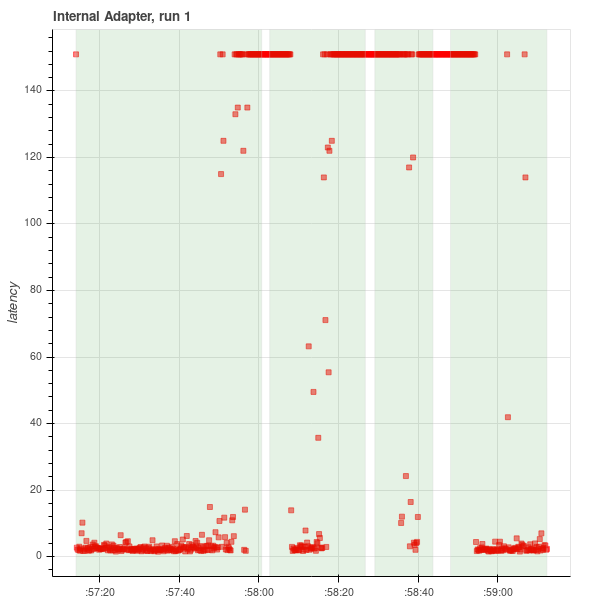
\includegraphics[width=\linewidth]{internal-1.png}
  \caption{Internal Adapter, run 1}
  \label{fig:int1}
\end{figure}

\begin{figure}
  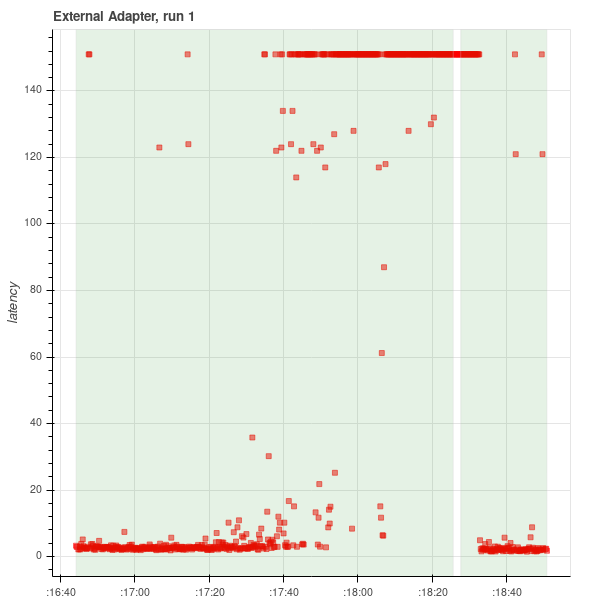
\includegraphics[width=\linewidth]{external-1.png}
  \caption{External Adapter, run 1}
  \label{fig:ext1}
\end{figure}

Additionally, we plotted the latency for each packet vs time on each run.
Shown are the first run of the internally-mounted Canakit adapter
(Figure \ref{fig:int1}), and the first run of the externally-mounted Canakit
adapter (Figure \ref{fig:ext1}). In these figures, the lightly shaded green
background represents the connection to an access point, with the white
indicating that the robot is not connected at that time. Response times along
the top of the graph indicate timeouts at 150 milliseconds or greater.

Meanwhile, for the watchdog testing, we took the following runs, eight each
with the watchdog enabled and with it disabled:

\begin{tabular}{ c | c | c }
  \centering
  Run & Enabled & Disabled \\ \hline
  1 & 10 & 198 \\
  2 & 13 & 144 \\
  3 & 15 & 156 \\
  4 & 15 & 192 \\
  5 & 14 & 198 \\
  6 &  8 & 156 \\
  7 &  8 & 192 \\
  8 &  4 & 168 \\
  \hline
  Average: & 10.9 & 176
\end{tabular}

For many of the runs with the watchdog disabled, the robot did not drive
straight ahead. Rather than estimating the distance that it travelled along
a curve, I instead opted to measure the straight line distance. Therefore,
measurements of the watchdog disabled should be regarded as minimums. On runs
where the robot drove straight, it consistently drove between 16 and 17 feet
(192-204 inches). 

For the measurements taken with the watchdog timer enabled (measuring 0 inches
to 20 inches) I measured with precision to the nearest inch.
For the measurements taken with the watchdog timer disabled (measuring 10 feet
or more), I measured with precision to the half foot, or six inches.


\section{Discussion}
From the data obtained here, we see that substantial improvements can be made
to the reliable control of the robot by simply improving the placement and
selection of the wireless adapter. Simply relocating the adapter to the outside
of the metal enclosure reduced packet loss by over ten percent in the tests
performed. Of note when looking at the figures provided, as well as the
additional graphs displayed on the GitHub repository\cite{uropgithub} is the
observation that the internally-mounted adapter disconnected from and
reconnected the wifi three times, as compared to the externally-mounted
adapter, which only disconnects and reconnects once.
Furthermore, this is also perhaps not an entirely fair comparison, as we are
comparing the best run of the internally-mounted adapter with the second-worst
run of the externally-mounted adapter, which just serves to exemplify the
effect that the shielding from the metal casing of the robot has on the
performance of the wireless adapters.

Further, we note that in these graphs, we see an increase in packet times as
some amount of time before the before all packets are lost and the connection
is dropped. Presumably, the increased loss (and therefore decreased goodput)
coorelate with decreasing signal strength. 

With regard to the watchdog, we notice much more dramatic improvements, with
stop times after signal is lost being an order of magnitude smaller. This will
lead to much easier regain of control after the signal is lost, and
drastically reduce the chances of damage happening to a robot when signal is
lost. During several of the test runs without the watchdog timer enabled, if 
the robot was not started perfectly straight, it had to be intercepted before
it ran into the wall or another obstacle, which was fairly likely with a
fifteen foot range. The watchdog effectively removed these demands from the
robot's operator.


\section{Conclusions}
Based on the data gathered over the course of the research, it appears that
the combination of improved hardware selection and placement with the added
improvement of a low-threshold watchdog timer to stop the robot in the absence
of a connection results in a stable robot connection. This serves to both
minimize the amount of interruption perceived in connection as the robot
navigates across the coverage regions of various access points on-campus, as
well as minimize the negative impacts that this interruption in a consistent
wireless control connection might otherwise provide. Together, these changes
as designed and tested provide a qualitatively much more pleasant user
experience for remote control and navigation of the robot, and, indeed,
driving after the changes were implemented was subjectively a much easier task
than previously.

However, driving the robot is still not a perfect experience, and there are
many avenues left for possible continued improvement.
At the physical layer, adding a second
network card would provide failover capability, and could potentially be
configured such that one network is always connected at a time, with packets
routed over the strongest (or over both). At the TCP/IP layers, tuning the
protocol parameters such as the TCP retry window could potentially make for
less delay and perceived latency when the robot does reconnect to the network.
Also, prioritizing the control data over the video with Quality-of-Service
scheduling would reduce packet congestion during periods of low goodput, such
as when there is a high signal-to-noise ratio. Finally, the methods we used
in this experiment could be repeated, but gathering additional data such
as the signal-to-noise ratio as reported by the wireless cards.

\bibliography{report}
\bibliographystyle{unsrt}

\end{document}
